\section{Product Perspective}
\label{sec:product_perspective}%

\subsection{Scenarios}
\label{subsec:scenarios}%

\textbf{Scenario 1: A biker uploads his latest path}

\textbf{Manuel Jimenez}, a cycling enthusiast, went on a biking trip around his hometown. He really liked the route and decided to store it on BBP. He opens the application, selects the storing a new path function and logs the origin, destination and other data from the trail. Because he is automatically logged in, he selects to upload the route to see if anyone wants to try it.

\bigskip
\textbf{Scenario 2: BBP detects a biker is on a route}

\textbf{Philip Thomas} is a college student that bikes every day to college. Since he regularly uses BBP, the app is logged in and tracks his location regularly. Since he always rides his bike to school, BBP detects his speed and assumes he is on his bike. One day, he changes the route because the road is closed. BBP recognizes the change of pathing and after the trip asks if he wants to update or add the path.

\bigskip
\textbf{Scenario 3: A biker reviews automatically detected potholes}

\textbf{Lucia Fernandez} is commuting to work. While she bikes, BBP automatically detects that she's moving at cycling speed and begins recording her trip. At one point, her phone vibrates unusually when she rides over a bump. The accelerometer flags a potential pothole.

When Lucia arrives at work, the app asks her to review the detected obstacles. She confirms one pothole and dismisses two false positives. BBP then asks if she wants to publish the updated path status.

\bigskip
\textbf{Scenario 4: A biker checks weather-enhanced statistics of a past ride}

\textbf{Jonas Richter} likes tracking his performance. After finishing a weekend ride, he opens BBP to view his stats. The system displays his distance, average speed, elevation changes—and also adds meteorological data retrieved automatically: cloudy weather, 12°C temperature, and moderate wind speeds during the ride.

Jonas reviews how the wind may have affected his total time and compares the results with other sessions.

\bigskip
\textbf{Scenario 5: A tourist searches for the safest path in a new city}

\textbf{Maria} is visiting Amsterdam and wants to bike from her hotel to a museum. She doesn't have a BBP account, but she can still browse public information. She enters her origin and destination into BBP.

The system returns three possible bike paths, each with a score based on surface quality, detected obstacles, and path safety. BBP highlights the highest-scoring path. Maria chooses that route and follows it on the map.

\bigskip
\textbf{Scenario 6: A biker manually updates a path's status after construction ends}

\textbf{David Bowell} regularly rides along a riverside road that recently underwent maintenance. He notices the pavement is now smooth and safe.

He opens BBP, selects the path from his saved routes, and manually updates its status from "requires maintenance" to "optimal." He confirms publishing the update.

\bigskip
\textbf{Scenario 7: A new user explores community paths for leisure rides}

A new registered user, \textbf{Aiden}, opens BBP to discover weekend cycling ideas. He browses the list of published paths contributed by the community. Each route shows distance, rating, path condition, and obstacles.

\subsection{Class Diagrams}
\label{subsec:class_diagrams}%

\begin{figure}[H]
    \begin{center}
        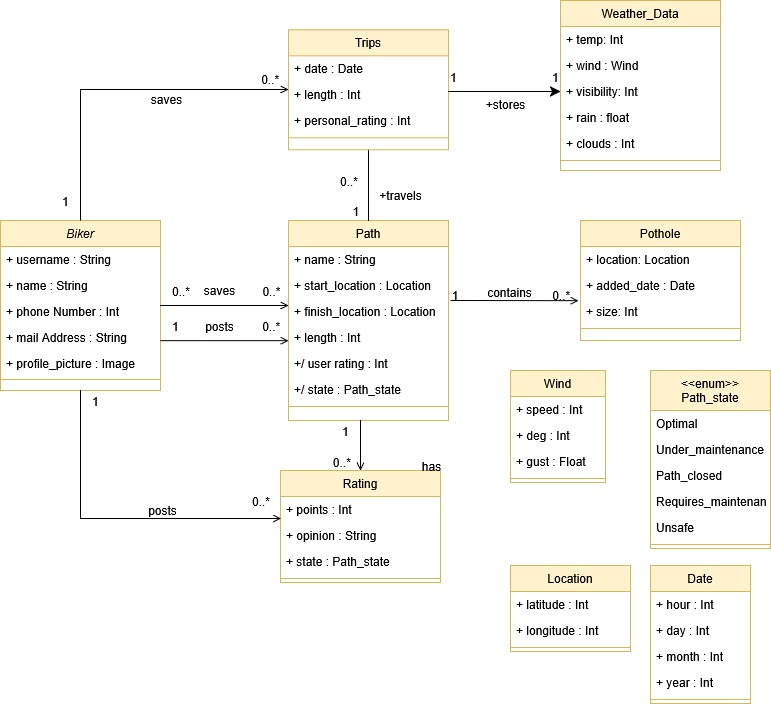
\includegraphics[width=0.9\linewidth]{Images/Diagrams/DomainClass.jpeg}
        \caption{Domain Class Diagram for Best Bike Paths}
        \label{fig:domain_class_diagram}%
    \end{center}
\end{figure}

In this Class Diagram we represent the entities and their relations in our system. The Best Bike Paths (BBP) system is a mobile application designed to enhance the cycling experience by providing a comprehensive platform for route discovery, recording, and sharing. The system serves two primary user groups: registered bikers who can record their trips, manually enter paths, allow automatic route detection, publish routes, rate paths, and access comprehensive statistics about their cycling activities; and non-registered users who can browse available paths, search for routes between two points, and view public information about path conditions and characteristics. The BBP platform serves as a centralized hub, collecting sensor data from mobile devices, processing route information, integrating weather data from external services, and providing route recommendations based on safety and quality scores.

The system's core entities include:
\begin{itemize}
    \item \textbf{Biker:} Represents registered users who can record trips, publish paths, and manage their cycling statistics.
    \item \textbf{Trip:} Stores comprehensive information about cycling trips, including duration, start time, rating, and optional weather data retrieved from external services.
    \item \textbf{Path:} Represents bike paths with attributes such as start and end locations, length, state (condition), rating, and associated potholes or obstacles.
    \item \textbf{Pothole:} Represents detected obstacles on paths, storing location coordinates, detection date, and size information.
\end{itemize}

The relationships between these entities enable the system to track user activities, maintain path information, and provide comprehensive route analytics. Bikers can have multiple trips, trips are associated with paths, and paths can contain multiple potholes, creating a rich data model that supports the system's functionality.

\subsection{State Diagrams}
\label{subsec:state_diagrams}%

The State Diagrams of the BBP system depict the various states and transitions for key system processes. These diagrams illustrate the lifecycle of trip recording, path managing and rating within the platform.

\begin{figure}[H]
    \begin{center}
        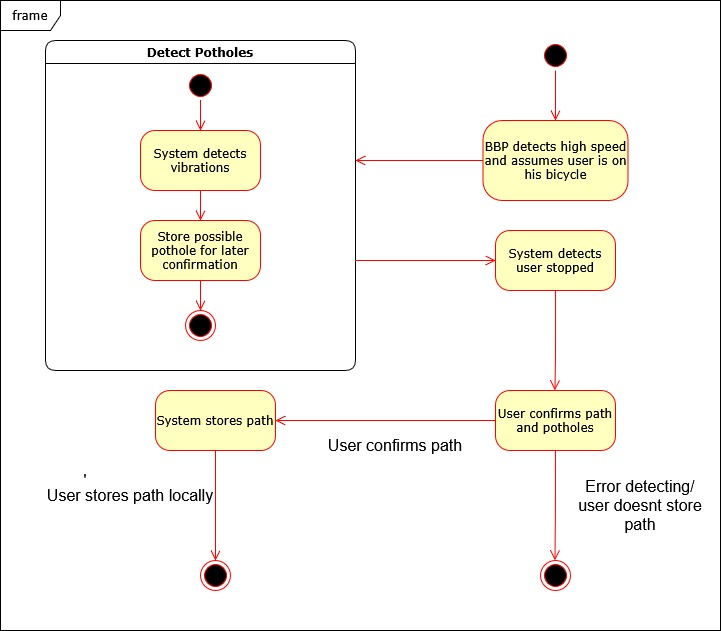
\includegraphics[width=0.8\linewidth]{Images/Diagrams/State_TripAutoRecording.jpeg}
        \caption{State Diagram for Automatic Trip Recording}
        \label{fig:state_diagram_1}%
    \end{center}
\end{figure}

This state diagram illustrates the process of automatic trip recording in the BBP system. It shows the various states that the system transitions through when automatically detecting and recording a user's cycling trip, including trip initiation, active recording, pothole recognition, and trip completion states. The diagram captures how the system handles automatic detection of cycling activity, GPS tracking, sensor data collection, and manages the user decision to confirm potholes and store or discard the path.

\begin{figure}[H]
    \begin{center}
        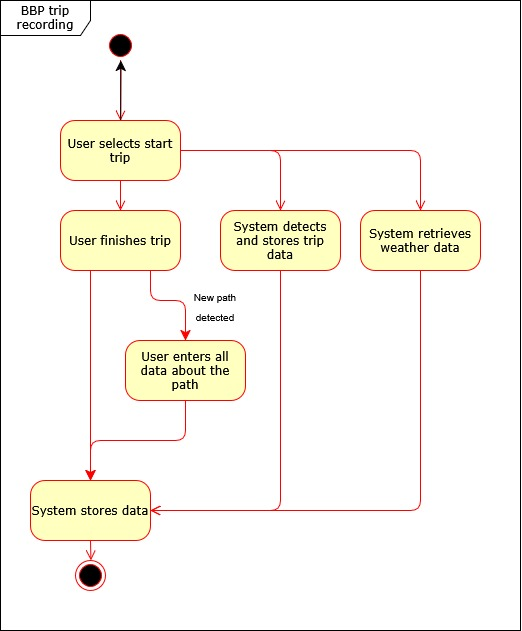
\includegraphics[width=0.8\linewidth]{Images/Diagrams/State_TripManualRecording.jpeg}
        \caption{State Diagram for Manual Trip Recording}
        \label{fig:state_diagram_2}%
    \end{center}
\end{figure}

This state diagram represents the states and transitions involved in manual trip recording. It depicts how users can manually initiate trip recording, enter path information if the path is not known, and manage the recording process. When a user starts a trip, it retrieves weather data and path data if available and stores and saves the information gathered during the trip. When the user finishes the trip, stores all information.

\begin{figure}[H]
    \begin{center}
        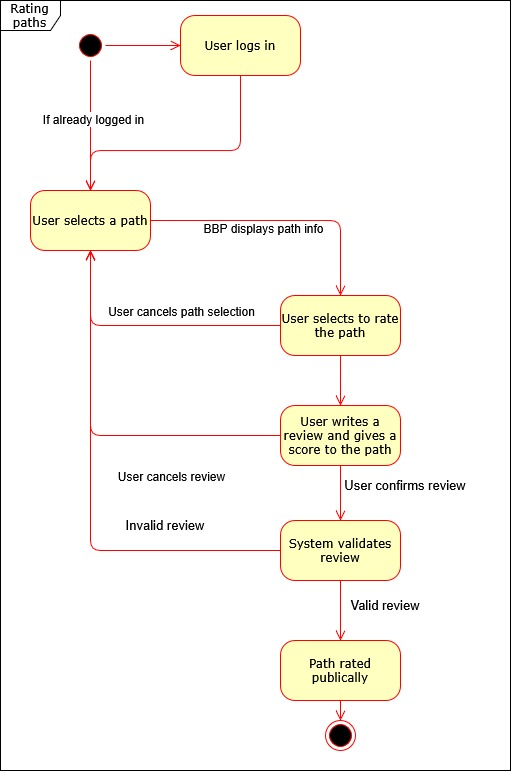
\includegraphics[width=0.8\linewidth]{Images/Diagrams/State_RatingPaths.jpeg}
        \caption{State Diagram for Path Rating Process}
        \label{fig:state_diagram_3}%
    \end{center}
\end{figure}

This state diagram models the path rating process within the BBP system. It illustrates the different states that occur when a user rates a path, including path selection, review creation, validation, and publication states. The diagram captures the workflow from when a user decides to rate a path through the submission and validation of their rating, showing how the system handles user input, review validation, and the final publication of ratings to the community.

\section{Product Functions}
\label{sec:product_functions}%

\subsection{Functions Available to All Users}
\label{subsec:functions_all_users}%

\begin{itemize}
    \item \textbf{Exploring Published Paths:} All users, regardless of registration status, can browse and explore the database of published bike paths. This includes viewing path details such as distance, rating, condition, and detected obstacles.
    \item \textbf{Finding Paths Between Two Points:} Users can query the system to find available bike paths connecting an origin and a destination. The system returns ranked path options based on computed scores that consider surface quality, obstacles, and safety factors.
\end{itemize}

\subsection{Functions Available to Registered Users}
\label{subsec:functions_registered_users}%

\begin{itemize}
    \item \textbf{Reviewing Past Trips:} Registered bikers can access comprehensive statistics and historical data about their previous cycling trips, including distance, duration, average speed, elevation changes, and weather conditions.
    \item \textbf{Posting New Paths:} Registered users can manually create and publish new bike paths, including origin, destination, and other relevant trail information.
    \item \textbf{Rating and Updating Paths:} Registered bikers can rate existing paths and provide updates about path conditions, such as changes in surface quality or the resolution of maintenance issues.
    \item \textbf{Automatic Trip Recording:} The system can automatically detect when a registered user is cycling, record GPS and sensor data, and propose detected paths and obstacles for user confirmation.
    \item \textbf{Path Status Management:} Registered users can save recorded trips, confirm or correct automatically detected paths and obstacles, and publish route or path status updates.
\end{itemize}

\section{User Characteristics}
\label{sec:user_characteristics}%

\subsection{User Groups}
\label{subsec:user_groups}%

The BBP system serves two primary user groups:

\begin{enumerate}
    \item \textbf{Registered Bikers:} Users who create accounts to access advanced features such as trip recording, path publishing, and personal statistics tracking.
    \item \textbf{Non-Registered Bikers:} Users who access the platform without registration to browse public path information and search for routes.
\end{enumerate}

\subsection{User Demographics, Restrictions and Frequency of Use}
\label{subsec:user_demographics}%

BBP is intended for anyone that enjoys riding a bicycle. There are no age, location or usage restrictions. The system is designed to accommodate:
\begin{itemize}
    \item \textbf{Demographics:} Cyclists of all ages and backgrounds, from casual riders to cycling enthusiasts, across various geographic locations.
    \item \textbf{Usage Frequency:} Users may access the platform daily for commuting purposes, weekly for recreational rides, or occasionally when exploring new areas.
    \item \textbf{Technical Proficiency:} The system is designed to be intuitive and accessible to users with basic skills using mobile devices.
\end{itemize}

\subsection{User Goals and Needs}
\label{subsec:user_goals_needs}%

All users want a useful app that helps them organize their biking trips. Specific needs include:
\begin{itemize}
    \item \textbf{Route Discovery:} Finding safe and enjoyable cycling routes in familiar or new areas.
    \item \textbf{Safety Information:} Access to information about path conditions, obstacles, and safety ratings.
    \item \textbf{Community Knowledge:} Leveraging the collective experience of the cycling community to discover and evaluate routes.
    \item \textbf{Performance Tracking:} For registered users, the ability to track and analyze their cycling activities and performance over time.
\end{itemize}

\section{Assumptions, Dependencies, and Constraints}
\label{sec:assumptions_dependencies_constraints}%

\subsection{Regulatory Policies}
\label{subsec:regulatory_policies}%

BBP complies with GDPR (General Data Protection Regulation). Personal data is used only for authentication, notification and profile management. Users may hide their identity with a username. The system ensures that:
\begin{itemize}
    \item User data is collected and processed in accordance with GDPR requirements.
    \item Users have control over their personal information and can manage privacy settings.
    \item Data is securely stored and transmitted using appropriate encryption and security measures.
\end{itemize}

\subsection{Domain Assumptions}
\label{subsec:domain_assumptions}%

The following domain assumptions are made for the BBP system:

\begin{enumerate}
    \item GPS access is granted by users on their mobile devices.
    \item Internet connectivity is available when users interact with the system.
    \item External services (weather API) respond correctly and provide reliable data.
    \item User data is valid and provided in good faith.
    \item Mobile devices have functioning sensors (GPS, accelerometer, gyroscope) that can provide accurate data.
    \item Users have basic familiarity with mobile applications and web interfaces.
\end{enumerate}

\subsection{Dependencies}
\label{subsec:dependencies}%

The BBP system depends on the following external components and services:

\begin{enumerate}
    \item Reliable web hosting services for the platform infrastructure.
    \item External weather API service for meteorological data integration.
    \item Secure database system for storing user data, paths, trips, and statistics.
    \item Mobile device sensors (GPS, accelerometer, gyroscope) for automatic trip detection and obstacle identification.
    \item Map services or APIs for displaying routes and geographic information.
    \item Authentication services to manage user logins and account security.
\end{enumerate}

\subsection{Constraints}
\label{subsec:constraints}%

The following constraints apply to the BBP system:

\begin{enumerate}
    \item Must comply with GDPR and data protection regulations.
    \item System must function correctly across major mobile operating systems (iOS, Android).
    \item Ensure system performance under high traffic and concurrent user loads.
    \item Provide compatibility across major web browsers for web-based access.
    \item Implement robust security standards for data handling and user privacy.
    \item Battery consumption must be optimized to minimize impact on mobile device battery life during trip recording.
    \item System must handle offline scenarios gracefully when internet connectivity is unavailable.
\end{enumerate}
